\section{La pensée en cycle de vie}
\label{sec:La pensée en cycle de vie}
Dans cette section nous traiterons des caractéristiques de la pensée en cycle de vie ainsi que des raisons de leurs élaborations.
Nous reprendrons le vocabulaire de la discipline avec une volonté d'accessibilité avant de faire plus tard la critique de la méthodologie.
Nous observerons l'évolution historique de la discipline depuis ses origines en en distinguant des caractères systémiques ayant contribué de façon à son état actuel.

\subsection{Quels fondements pour l'ACV~?}
L'analyse en cycle de vie, multicritère, résulte de la volonté d'éviter le report d'impact.

Tout d'abord, le report qui nomme la méthode, éviter le transfert d'impact d'une phase de vie d'un produit à une ou plusieurs autres de ses phases de vie.
\begin{figure}[htbp]
\centering
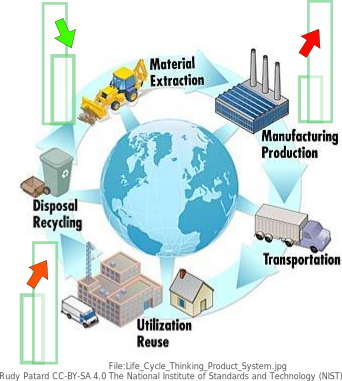
\includegraphics[width=0.5\textwidth]{/home/rudy/Documents/rudy/01_These/11_production/01_COMMUNICATION/02_PRESENTATION/BEAMER/images/report_impacts_phases_vie.pdf}
\caption{Illustration du report d'impacts entre phases de vie.}
\label{fig:report_impacts_phases_vie}
\end{figure}
\figbox{Sur la figure~\ref{fig:report_impacts_phases_vie}, une action de réduction d'un impact sur une phase de vie du produit (l'extraction de matières premières), génère une hausse des impacts sur deux autres phases (en fabrication et en utilisation).}
\exbox{
L'électrification d'une motorisation va affecter la phase d'utilisation.
Les émissions de combustion d'un moteur thermique se situent à la localisation du moteur alors que celles de la production d'électricité se trouvent sur les sites de production.
La nature des émissions pour la production et le traitement en fin de vie d'un moteur thermique, du réservoir associé et de son carburant seront différentes de celles de la fabrication d'un moteur électrique, de la batterie associée et de la source d'électricité.
}

Ceci nous conduit au second type de report, celui en \emph{nature d'impact}.
\begin{figure}[htbp]
\centering
\includegraphics[width=0.5\textwidth]{/home/rudy/Documents/rudy/01_These/11_production/01_COMMUNICATION/02_PRESENTATION/BEAMER/images/report_impacts.pdf}
\caption{report en nature d'impact.}
\label{fig:report_impacts}
\end{figure}
\figbox{Sur la représentation~\ref{fig:report_impacts} est illustré un transfert entre indicateurs sur les ressources et indicateurs sur la santé humaine.
Il s'agit simplement d'une illustration à visé pédagogique, le nombre de dimension étant bien supérieur.}
\exbox{
Les travaux sur les motorisations thermiques et la réduction des émissions de $CO_2$, de $NO_x$ et de particules sont intéressantes sur ce point.
Alors qu'une combustion \emph{complète} libère de la vapeur d'eau et du dioxyde de carbone, différents points de fonctionnement et divers carburants et mélanges avec comburant produisent une gamme variée d'émissions.
Il en résultent de nombreux compromis possibles entre l'émission de particules et de gaz générant du forçage radiatif.
}

La diversité des émissions et de leurs effets produit une autre caractéristique de l'ACV, l'agrégation des impacts.
\exbox{
Plusieurs substances différentes peuvent avoir un même effet.
Par exemple~: la vapeur d'eau, le dioxyde de carbone, le méthane, sont des \gls{GES}, au même titre que le perfluorobutane, le cis-perfluorodecalin, le dimethyl ether, l'hexafluoroethane, le perfluoropropane\ldots mais qui chacun auront une durée et une ampleur d'effet différent.
De même une même substance peut avoir plusieurs effets.
%\footnote{ Plus de détails sont disponibles dans la section d'analyse des méthodes d'impacts (\ref{sec:impactsmethods})}.
Le chloroforme est caractérisé dans l'ILCD2011 (méthode d'impacts européenne) pour son effet sur les impacts de changement climatique ; de toxicité humaine, canérigène et non-cancérigène ; de formation de particule ; de formation d'ozone photochimique ; d’écotoxicité aquatique en eau douce.
Nitric oxide, Nitrogen dioxide, Nitrogen oxides,
les oxydes d'azotes sont caractérisés (ILCD2011) pour la formation d'ozone photochimique, l'acidification et l'eutrophisation terrestre et marine.
%Le protoxyde d'azote. Dinitrogen monoxide, n'a qu'un facteur et porte sur le réchauffement climatique.
}
Ainsi plus qu'aux substances, c'est à leurs effets qu'a trait l'information produite par l'ACV
\footnote{L'inventaire collectera évidement les substances, mais cette activité relève de l'analyse de procédé plus que de l'analyse en cycle de vie, bien que la seconde (ACV) nécessite la première (analyse de procédé).}.
Cette structuration vers les effets a pris en ACV deux courants qui tendent à se rejoindre.
Les méthodes orientées impacts et les méthodes orientées dommages relèvent d'un degré d'agrégation variable qui cherche un équilibre entre maîtrise de l'incertitude et la capacité de faire sens pour le décideur. %(\textit{cf.} section \ref{sec:methodesdimpacts})
\begin{figure}[htbp]
\includegraphics[width=\textwidth]{/home/rudy/Documents/rudy/01_These/11_production/01_COMMUNICATION/02_PRESENTATION/BEAMER/images/ILCD_principe_3_niveaux_information.png}
\caption{ILCD principe 3 niveaux information modified}
\label{fig:ILCD_principe_3_niveaux_information.png}
\end{figure}
\figbox{
La figure~\ref{fig:ILCD_principe_3_niveaux_information.png}, représente les agrégations midpoints et endpoints des indicateurs d'impacts en ACV.
La multiplicité des impacts par substance et la multiplicité des dommages par impacts est représentée par les flèches.
En ajout à la figure initiale nous avons représenté l'accroissement de l'incertitude au fil du déroulement des mécanismes environnementaux.}

Puisque l'ACV vise la sélection d'alternatives au sein de systèmes humains (décisions), il est tout à fait logique qu'elle se soit déployée avec l'intégration de dimensions sociales et économique, donc politiques.
%\colorbox{yellow}{ILCD stepwise extansion}
Ces caractéristiques combinées poussent la méthode dans une tendance holistique.
Puisqu'il n'est pas jugé a priori d'une importance supérieure d'un instant ou d'une nature d'impact, la méthode cherche à \emph{tout} circonscrire.
Puisque les activités humaines et éco-systémiques sont fortement et planétairement liées, l'aire d'étude porte rapidement sur tout le globe.

\subsubsection{Vocabulaire de base}
\label{subsubsec:Vocabulaire de base}
Nous nous contenterons de la description du vocabulaire tel qu'employé actuellement.
D'autres représentations sont possibles.
Une en sera donnée chapitre~\ref{chap:ACV, la (re)conception d'un outil}, plus particulièrement au point~\ref{par:Distanciation à la représentation classique de l'ACV}.
Nous nous attacherons dans cette présentation à identifier des origines historiques sur les termes afin de comprendre les racines méthodologique de l'\gls{ACV}.

\begin{figure}[htbp]
\includegraphics[width=\textwidth]{/home/rudy/Documents/rudy/01_These/11_production/01_COMMUNICATION/figures/cycle_ILCD_jrc_modif_EN.pdf}
\caption{Des flux qui comptent. Graphique Cycle ILCD modifié \cite{european_commission_ilcd_2010}.}
\label{fig:cycle_ILCD_jrc_modif}
\end{figure}
%\keybox{
\figbox{Dans la figure~\ref{fig:cycle_ILCD_jrc_modif}, nous posons un ensemble de mots clefs de la discipline.
Les \glspl{fluxelementaire} traversent la ligne pointillé démarquant \gls{technosphere} et \gls{ecosphere} (ou \gls{biosphere}).
Les \glspl{fluxproduit} s'échangent entre les étapes du cycle de vie, de 'l'extraction des ressources' à 'la fin de vie'.
Au centre de l'étude se trouve la clef de comparaison des alternatives, l'\gls{UF}.
Son unicité garanti la comparabilité des alternatives.
La délivrance de l'\gls{UF} à l'utilisateur est quantifiée par le \gls{fluxdereference}.
Chaque alternative comparée l'est sur la base de la même quantité du \gls{fluxdereference}.
L'ensemble des autres flux sont 'mis à l'échelle' pour conserver cette unicité de l'\gls{UF}.}
%}
\paragraph{La \gls{technosphere}} La recherche sur ce terme nous a conduit à des pistes interessante dans l'histoire de l'ACV. La \gls{technosphere} est le milieu des interactions humaines.
Absent du \citetitle{markandya_dictionary_2001}, l'\gls{ILCD} la définit au travers des flux élémentaires\footnote{\blockcquote[traduction]{european_commission_ilcd_2010}{
La frontière technosphère / écosphère peut donc être plus convenablement définie par la définition de flux élémentaire.
%The boundary technosphere / ecosphere can hence be more suitably be defined by defining the elementary flow.
}} (voir ci-après).
La complexité de sa définition n'est pas surprenante lorsque l'on observe sa formation par délimitation des voisins.
\blockcquote[traduction]{bruni_cognitive_2011}{Il est difficile de retracer l'origine exacte du terme "technosphère".
Il est clair cependant que le concept est un dérivé de ceux, complémentaires, de Eduard Suess et Vladimir Verdnasky de "bio-sphère" et de la notion de Teilhard de Chardin de "noosphère".}
%It is hard to trace back the original coining of the term “technosphere”. It is clear however that the concept is a derivative of Eduard Suess and Vladimir Verdnasky’s complimentary concept of “bio-sphere” and Teillard de Chardin’s notion of “noosphere”.
%}

Identifié par \citeauthor{bruni_cognitive_2011,} comme originaire de Michel \textsc{Batisse} (que nous n'avons pu vérifier), l'auteur la définit comme suit~:
\blockcquote[traduction]{bruni_cognitive_2011}{
Immédiatement au-dessus de la biosphère, et maintenant l'entourant entièrement, est un niveau plus élevé d'organisation, qui n'est devenu important que récemment, et qui peut être appelé la technosphère.
Elle est non seulement composée des usines, des barrages et des champs irrigués, mais aussi de tout le canevas des faits technologiques et des caractéristiques de natures physiques, chimiques ou biologiques (Batisse, 1973).}
%Immediately above the biosphere, and now surrounding it entirely, is a higher level of organization, which has become important only recently, and which can be called the technosphere. This is not only made up of the factories, the dams and the irrigated fields, but also the whole canvas of technological facts and features of a physical, chemical or biological nature (Batisse, 1973)
%}
De façon intéressante, dans cette représentation la techno-sphère se développe sur et autour de la biosphère ("surrounding it").
C'est une représentation opposée à celle de l'ACV, d'une technosphère \emph{entourée} d'\emph{éco}sphère.

Nous avons pu remonter dans l'histoire de ces termes jusqu'en 1968 (\citeauthor{milsum_technosphere_1968}, \citetitle{milsum_technosphere_1968}~\cite{milsum_technosphere_1968}).
Mais c'est en 1969 que l’occurrence la plus significative fut trouvée~\cite{iugg_i.u.g.g._1969}.
Parce que les termes employés sont significatif par leur similarité au langage de l'ACV actuelle, voici un extrait, sans traduction, du rapport.
\blockcquote{iugg_i.u.g.g._1969}{The ad hoc Committee has considered in detail the following ways in which man is altering the environment:\\
1. Increase in human population density.\\
2. Increase in \textbf{atmospheric carbon dioxide} from the combustion of fossil fuels.\\
3. Increase in turbidity (\textbf{particulate} content) of the atmosphere.\\
4. Pollution of the \textbf{oceans} and \textbf{coastal waters}.\\
5. \textbf{Radioactivity} in the atmosphere, natural waters, soils and living organisms.\\
6. \textbf{Deliberate and inadvertent modification of the atmosphere}, including the effects of cloud seeding and jet contrails.\\
7. Effects of introduced species.\\
8. Pressures on available \textbf{water resources}.\\
9. \textbf{Eutrophication} of international waters.\\
10. \textbf{Soil erosion and destruction}.\\
11. \textbf{Noise} as a pollutant.\\
12. Dissemination of \textbf{pollutants in air, soils, water} and living organisms (including Industrial and domestic \textbf{wastes}, pesticides, reactions In the atmosphere, biological molecules).\\
13. \textbf{Degradation of natural ecosystems with the loss of gene pools}.\\
14. Thermal pollution (atmosphere and international waters).
%There Is a wide variability in the scale of these effects, In the urgency of environmental threats, in the ways in which man could be affected.
%The Committee considered these facts, and also took note of the other International organizations which are Involved.
%The principal conclusion of the Committee Is that ICSU has a responsibility to provide objective scientific leadership In this field,
[\ldots] The ad hoc Committee recommends that ICSU set up a \textbf{Scientific Committee on Problems of the Environment} (SCOPE),
%[\ldots]
which would \textbf{bring together the various disciplines}, and which, through Its Commissions, would be responsible for the promotion of \textbf{environmental monitoring}, \textbf{evaluation of the effects of environmental disturbance} , \textbf{simulation modelling and predictions}, and the study of the \textbf{social effects} of man-made change in the environment.
%It Is recommended that SCOPE be provided with a secretariat which should be developed into as International Centre for the Environment.
%The ad hoc Committee recommends that SCOPE and the International Centre for the Environment cooperate fully with other groups, outside of ICSU, including all Involved UN Agencies, regional intergovernmental bodies, and international nonM-BM--governmental bodies.
[\ldots]
The commissions should in the first instance include:
(i) commission on monitoring,
\textbf{(ii) commission on biosphere and technosphere evaluation,}
(iii) commission on quantitative predictions,
(iv) commission on \textbf{social and economic evaluation}.}
%cat -v pour netoyer le fichier.
%clean with emacs ? C-M-s pas encore compris, but : ne garder que de l'ASCII
%http://tex.stackexchange.com/questions/4268/inputenc-error-unicode-char-u8-error-while-trying-to-write-a-degree-symbol#4270
Il semble peu probable que ces commissions se soient établies sans antériorités des termes et des recherches qui en composent les noms et activités.
Vous constaterez comme moi que la quasi totalité des termes courant de la pensée en cycle de vie s'y retrouve.
Pour autant nous n'y trouvons pas les mécanismes d'évaluation.
%, même l'inclusion de la nuisance du bruit, toujours en discussion pour l'intégration aux méthodes d'impact aujourd'hui.

%\footnote{
%%Le \href{https://books.google.com/ngrams/graph?content=technosphere&year_start=1800&year_end=2000&corpus=15&smoothing=3&share=&direct_url=t1\%3B\%2Ctechnosphere\%3B\%2Cc0#t1\%3B\%2Ctechnosphere\%3B\%2Cc1}{NgramViewer de technosphere} (bien que revoyant à 1938) renvoi à Milsum, J. H. (1968) "Technosphere, Biosphere and Sociosphere", General Systems, 13. (il est plus probable que Milsum ait écrit en 68 qu'en 38).
%Des références à l'IUGG International Union of Geodesy and Geophysics et à l'ICSU International Council of Scientific Unions (1965 -66 -68 -69), référence sur lequelles nous n'avons pas pu mettre la main. Des requêtes ont été adressées à l'ICSU et l'IUGG.}


\paragraph{La \gls{biosphere} ou l'\gls{ecosphere}.}
Si la littérature semble plus employer la première que la seconde\footnote{\href{https://books.google.com/ngrams/graph?content=biosphere,ecosphere&year_start=1800&year_end=2008}{lien vers ngrams comparatif~: ecosphere, biosphere}} \footnote{\href{https://books.google.com/ngrams/info}{Lien vers les explications des ngrams}.}, l'ILCD se réfère à l'\emph{éco}-sphère.
Ce choix se comprends au travers des dimensions observées en ACV.
L'épuisement des ressources n'est pas du domaine du vivant.
Mais suivant les définitions employées de biosphère (voir plus bas), ce choix n'est pas sans contradiction.
L'\gls{ecosphere} n'est pas définie directement, mais comme la techno-sphère, sa définition résulte de celle du flux élémentaire.
Une représentation en est donnée \cite[figure 13 p.99]{european_commission_ilcd_2010}.
Elle y est périphérique à la techno-sphère.
La définition ACViste a ceci de particulier que dans son approche actuelle, l'écosphère, par complément de la techno-sphère, est l'espace où il n'y a pas d'intervention humaine, or ceci relève d'une inconsistance lorsqu'elle intègre l'homme dans sa 'matière vivante' avec les impacts attenants.

La double définition de biosphère du \citetitle{markandya_dictionary_2001}, présente celle-ci à la fois comme la région de la terre où la vie existe et les éléments constitutifs de la vie elle même (matière, énergie, information).

\paragraph{Le \gls{fluxelementaire}} est un concept clef pour les définitions en ACV. Un flux élémentaire est d'après l'ILCD une \blockcquote[traduction et synthèse d'un extrait de "Terms and concepts" p.94]{european_commission_ilcd_2010}{substance unique ou énergie extraite de, respectivement émise dans, l'\gls{ecosphere}, sans transformation humaine, précédente, respectivement suivante.}
%“single substance or energy entering the system being studied that has been drawn from the ecosphere without previous human transformation, or single substance or energy leaving the system being studied that is released into the ecosphere without subsequent human transformation”.
%material or energy entering the system being studied that has been drawn from the environment without previous human transformation, or material or energy leaving the system being studied that is released into the environment without subsequent human transformation”}
Puisque la définition de l'éco-sphère intervient dans la définition donnée par l'ILCD du flux élémentaire et réciproquement, la reformulation qui nous semble la plus pertinente est~:
Échange d'une substance qui, soit n'a jamais subi intentionnellement d’interaction humaine antérieure, soit n'en subit plus ultérieurement.

Ceci permet donc la définition itérative de la frontière techno-éco sphère sans l'appel de l'un des deux concepts et sans contradiction avec les impacts (interaction non-intentionnelle).
La notion primordiale est donc l'interaction humaine intentionnelle.
Les autres notions en sont des dérivations.
\paragraph{Le \gls{fluxproduit}} est définit par l'ILCD de la façon suivante~:
\blockcquote[traduction p.22]{european_commission_ilcd_2010}{
Un des flux de co-produits dans l'inventaire d'un procédé ou système qui accompli la fonction du procédé / du système.
Voir également~: Flux non-fonctionnel.
%One of the (co-)product flow(s) in the inventory of a process or system that fulfils the processus' / system's function. See also: Non-functional flow
}
\footnote{Inconsistance du référentiel méthodologique : \blockcquote[p.22]{european_commission_ilcd_2010}{Non-functional flow: Any of the inventory items that are not (co-)product flows. E.g. all emissions, waste, resources \textbf{but also} input flows of processed goods and of services.}
Le lecteur comprendra que si un flux est extrait de la biosphère pour \emph{servir} sous forme de biens et services, il recèle un caractère utile et \emph{fonctionnel}.}

\paragraph{Le \gls{fluxdereference}}, ou flux référentiel, ou encore reference flow pour les anglophones.
\blockcquote[Traduit de Terms and concepts: Function, functional unit, and reference flow p.60]{european_commission_ilcd_2010}{Le flux de référence, finalement, est le flux (ou les flux en cas de procédés multifonctionnels) auquel tous les autres flux entrant et sortant se rapportent. Il est celui qui réalise l'unité fonctionnel~: Le flux de référence peut être directement exprimé en relation à l'unité fonctionnelle.}
%
%The reference flow, finally, is the flow (or flows in case of multifunctional processes) to which all other input and output flows (i.e. all elementary flows and non-reference product and waste flows) quantitatively relate. It is realising the functional unit: The reference flow can be expressed in direct relation to the functional unit (e.g. “Complete coverage of 1 m 2 primed outdoor wall for 10 years at 99.9 \% opacity with paint A") or in a more product-oriented way (e.g. "0.67 l paint A").
%}

Pour plus de définition, nous renvoyons le lecteur à \citetitle[section 3 Key definitions]{european_commission_ilcd_2010} et aux encarts 'Terms and concepts'~\cite{european_commission_ilcd_2010}.

\subsubsection{L'Analyse du Cycle de Vie en détails}
L'analyse en cycle de vie comporte 4 étapes selon l'\gls{ISO}, 5 selon l'\gls{ILCD}.
\begin{figure}
\centering
\includegraphics[width=\textwidth]{/home/rudy/Documents/rudy/01_These/11_production/01_COMMUNICATION/figures_extraites/LCA-phase.pdf}
\caption{Cadre de travail et phase de l'ACV~\cite{european_commission_ilcd_2010}.}
\label{fig:LCA-phase}
\end{figure}
\figbox{Les flèches alternées de la Fig.~\ref{fig:LCA-phase} représentent le caractère itératif de la méthode.
Les applications de la méthodologies sont listés à droite des étapes qui sont~: la définition des buts, définition du périmètre, production et analyse de l'inventaire, caractérisation et interprétation.
%\exbox{test}
}
\paragraph{Itérative},
\blockcquote[]{european_commission_ilcd_2010}{
Dispositions~: 4 L'approche itérative pour l'ACV\\
I) Possible - Aperçu de l'approche itérative~: Il est recommandé de prendre une approche itérative pour l'étude ICV / ACV% (pour plus de détails voir le chapitre 2.2.4)
%Provisions: 4 The iterative approach to LCA
%I) MAY - Overview of iterative approach: It is recommended taking an iterative approach to the LCI/LCA study (for more detail see chapter 2.2.4)
\ldots
}
% nltk 'iterative' occurences ?
\paragraph{Définition du but de l'étude.}
Cette étape détermine la question de recherche, l'objectif à atteindre par sa résolution.
C'est cette réflexion qui détermine l'\gls{UF} ainsi que les alternatives qui seront étudiées.
Remarque~: L'expression du but peut précéder la réalisation d'une \gls{AF} des objets d'études.
Mais il est à prévoir qu'en l'absence d'\gls{AF} préliminaire, l'\gls{UF} sera révisée à son issue.
\paragraph{Définition du périmètre.}
Suivant la définition de l'\gls{UF}, un nombre variable de procédés seront nécessaires pour satisfaire sa délivrance.
Dans l'approche actuelle, le but de l'étude et les alternatives considérées peuvent modifier l'inclusion ou l'exclusion dans le périmètre.
Tout périmètre valide est celui qui ne modifie pas les conclusions de l'étude conformément à son but.
\exbox{Exemple d'exclusion de périmètre considéré comme praticable.
La confrontation pour le choix entre deux alternatives mettant en œuvre un système commun et ce dans les mêmes proportions permettra à l'analyste d'exclure du système étudié ces systèmes dont la comparaison (différence) est connue d'avance car nulle.
L'effet sur le résultat invite donc à l'exclusion.
Toutefois, le constat de l'équilibre permettant l'exclusion se fait à posteriori.
Sont intérêt est donc limité.}
\paragraph{Réalisation et analyse de l'inventaire.}
La réalisation de l'inventaire concerne la modélisation du système socio-technique délivrant l'\gls{UF}.
Le travail d'inventaire consiste en la collecte et le traitement des données d'observation du système étudié.
Partant des procédés identifiés au périmètre initial (satisfaisant la délivrance de l'\gls{UF}), il s'agit de renseigner l'ensemble des flux, produits et élémentaires, entre l'ensemble des procédés dans la \gls{technosphere} ainsi qu'entre ces procédés et la \gls{biosphere} sous ses diverses compartimentations.
Son résultat est l'\gls{ICV}.
L'étape cristallise les problématiques de multifonctionnalité et de disponibilité des données, traitées respectivement au \ref{chap:Multifonctionnalité} et au \ref{chap:Recherche Libre}).
Dans sa conception actuelle, cette étape est concentrée sur les données de la \gls{technosphere}.
La modélisation des systèmes environnementaux étant réduite à l'utilisation de méthodes d'impacts, nous la traitons dans l'étape suivante.

\paragraph{Évaluation des impacts.}
Cette étape est également dénommée caractérisation.
Sur la base de l'ensemble des flux élémentaires collectés et affectés à leurs compartiment respectifs (air, eau, sol et sous-catégorisations), les effets sur les mécanismes environnementaux sont évalués à diverses échelles (tel que représenté Fig~\ref{fig:ILCD_principe_3_niveaux_information.png}).
Les méthodes d'impacts sont observées section~\ref{sec:LCIAM}
Il résulte de cette étape une liste d'indicateurs caractérisés.
\paragraph{Interprétation.}
Souvent détaillée pour l'interprétation finale, il est à noté qu'en figure~\ref{fig:LCA-phase} elle apparaît bien à chacune des étapes.
Avant le traitement de de la caractérisation, l'interprétation vise donc à contrôler l'ensemble des étapes précédentes à chaque pas (le périmètre respectivement au but, l'inventaire respectivement au but et au périmètre etc.).

Le cœur de l'étape d'interprétation consiste en la réduction des données sous une forme exploitable pour la décision.
Le regroupement en aires de protection (indicateurs de dommages) ou en score unique font partie de ce traitement.
Les opérations actuellement détaillées dans la méthodologie portent sur la pondération et la normalisation.

%Il s'agit ci-après des pondérations réalisées dans le cadre d'études liées à l'environnement.
Une synthèse de la classification de \citeauthor{rowley_aggregating_2012} reprenant Finnveden, 1999~\cite{finnveden_critical_1999}; Lindeijer, 1996; Hofstetter, 1996 et POWELL(1997)~\cite{powell_approaches_1997} a été faite.
L'interprétation se fait donc~:
\begin{itemize}
\item Par sélection (équipondérée). (monocritère ou en nombre réduit les autres étant négligés)
\item Par monétarisation~:
%\footnote{avec ici la distinction faite par \citeauthor{powell_approaches_1997} entre coût du contrôle environnemental et coût du dommage environnemental.}
\begin{itemize}
\item Par coût du contrôle environnemental. 
Le poids est attribué suivant le coût représenté par les mesures de contrôle d'émission de la substance.
\item Par coût du dommage environnemental.
Le poids est attribué suivant l'\emph{estimation} du coût engendré par les dommages liés à l'émission de la substance.
Par exemple, la méthode basée sur la ``volonté à payer'' des individus pour la protection ou la réparation.%
%\footnote{HARRIBEY dans\cite{harribey_richesse_2013} précise que les valeurs monétaires estimées l...
\end{itemize}
\item Par Distance à la cible. Les cibles peuvent être dérivées de réglementations ou de limites jugées utiles pars un corps tiers et estimées scientifiquement~\cite{seppala_meaning_2001}.
\item Par panel. Les travaux de \citeauthor{myllyviita_impact_2014} portent sur l'étude de la pondération par panel. (Où : Comment un groupe de personnes attribue des poids aux indicateurs~?)~\cite{myllyviita_impact_2014}.
\end{itemize}

Ces opérations sont critiquées section~\ref{chap:Jugements et Multi-dimensionnalité}.
Cette étape est évidement centrale dans notre travail d'intégration du jugement dans la méthodologie.


\subsubsection{Synthèse des caractéristiques méthodologiques spécifiques}
{Itérative} et {Multi-critère} dans sa quête holistique, l'\gls{ACV} se déploie par étapes pour
(i) fixer ses objectifs et son cadre décisionnel,
(ii) établir sa clef de comparaison qu'est l'\gls{UF},
(iii) comptabiliser ses échanges de \glspl{fluxproduit} dans la \gls{technosphere} et de \glspl{fluxelementaire} avec la \gls{biosphere},
(iv) puis évaluer les effets sur les mécanismes environnementaux en caractérisant des indicateurs d'impacts,
(v) et enfin faire l’interprétation de cette caractérisation.

Nous venons donc de voir les caractéristiques actuelles et les fondements de l'\gls{ACV}.
Observons maintenant leurs causes et origines.

\subsection{L'origine de l'ACV}
\label{subsec:L'origine de l'ACV}

Nous avons cherché l'origine de l'évaluation en cycle de vie dans le premier numéro du journal international éponyme.
\citeauthor{hunt_lca-_1996} dans \citetitle{hunt_lca-_1996}, attribuent l'origine de l'ACV au travail de
\blockcquote{hunt_lca-_1996}{Harry E. TEASLEY, Jr.} en 1969, travaillant pour la célèbre marque de boisson pétillante caféinée.

\citeauthor{boustead_lca_1996} dans \citetitle{boustead_lca_1996}, situe également les premiers pas de ce qui deviendra l'ACV par l'évaluation des matériaux d'emballage et notamment le packaging en verre des boissons avec la méthode d'énergie cumulée.
Cette introduction est fort intéressante en ce qu'elle dévoile la mixité et proximité des activités économiques, académiques et politiques.

\citeauthor{boustead_lca_1996} nous offre en effet un tableau comprenant~:
\begin{itemize}
\item Des groupes de pression (Amis de la Terre) s'opposant aux groupes industriels~\footnote{
\blockcquote[traduction]{boustead_lca_1996}{
Les Amis de la Terre ont renforcé leur position par le déversement d'un camion chargé de bouteilles vides non récupérables sur le seuil du siège social de Schweppes à Londres.
%Friends of the Earth reinforced their stance by dumping a truck-load of empty non-returnable bottles on the doorstep of Schweppes head office in London
}
},
\item Des groupes des industriels cherchant défenses et cautions scientifiques~:
%\footnote{
\blockcquote[traduction]{boustead_lca_1996}{
La fédération des producteurs de verre a décidé qu'ils avaient intérêt à obtenir des informations quantitatives définitives avec lesquelles monter leur défense.
%the Glass Manufacturers Federation decided that they had better get some definitive quantitative information with which to mount their defence.
}
%},
\item La Recherche leur fournissant `expertise et caution' scientifique contre du financement~:
%\footnote{
\blockcquote[traduction]{boustead_lca_1996}{
L'\textit{Open University} était une institution nouvelle et avait peu de fonds pour la recherche.
Donc, l'exécution des travaux de sous-traitance fournirait des fonds pour notre recherche universitaire.
%the Open University was a new institution and had few research funds. So carrying out contract work would provide funds for our academic research.
}
%},
\item L'inter-relation au contexte international et aux crises politico-économiques (73 notamment)~:
%\footnote{
\blockcquote[traduction]{boustead_lca_1996}{
Il s'était donc trouvé que lorsque la première crise du pétrole frappa, nous poursuivions une double approche à l'analyse de l'énergie.
%So it was that when the first oil crisis hit, we were pursuing a twin-track approach to energy analysis.
}
\footnote{Ladite crise de 1973, se situe entre 71 et 73 selon que l'on considère le pic de production américain, la modification des propriétés de conversion du dollar, ou l'embargo de l'OPEP.}
%}.
Les lecteurs attentifs ou les experts du domaine n'auront pas raté la proximité chronologique du rapport \citetitle{meadows_limits_1972}.
\item Le contraste du rapport aux données selon les intérêts gouvernementaux entre économistes et écologistes~:
%\footnote{
\blockcquote[traduction]{boustead_lca_1996}{
Dans les premiers jours un problème majeur était le manque de données primaires fiable d'origine industrielles et nous avions l'habitude de regarder avec envie nos cousins économistes qui ont accès aux vastes exercices de suivi effectués aux frais du gouvernement.
%In the early days one major problem was the shortage of reliable industry based, primary data and we used to look with envy at our economist cousins who had access to the vast monitoring exercises carried out at government expense.
}
%}.
\end{itemize}
Un trait intéressant de ces retours historiques est d'observer l'omniprésence dans un espace de `recherche', d'organismes dépendant de contrat avec des parties prenantes à caractère industriel, commercial et lucratif.
Un état de fait qui a perduré jusqu'ici.

C'est toutefois dehors de cette parution nous trouvons des éléments de similarité à l'ACV des plus intéressants.
Si intéressants que nous n'y voyons rien d'autre que les origines de l'ACV.
Nous avons déjà vu dans la section sur le vocabulaire l’extrême similitude quant au SCOPE et ses commissions (en 69) (\ref{subsubsec:Vocabulaire de base}).
En \citeyear{leontief_environmental_1970}, dans son article \citetitle{leontief_environmental_1970},  \citeauthor{leontief_environmental_1970} décrit une approche par "entrée-sorties" dont le vocabulaire ne manquera pas non plus de similitude à l'ACV.

\blockcquote[traduction]{leontief_environmental_1970}{
La pollution est un co-produit des activités économiques habituelles\footnote{Vous noterez bien, la polution est une co-production (original~: POLLUTION is a by-product)}.
Dans chacune de ses multiples formes, elle est reliée de façon mesurable à une consommation particulière ou un procédé de production.
La quantité de monoxyde de carbone relâchée dans l'air porte, par exemple, une relation définie à la quantité de carburant brûlée par divers types de moteurs d'automobiles ; le rejet d'eau polluée dans les courants et les lacs est directement lié au niveau de production d'acier, de papier, de textile et de toutes les autres industries utilisant l'eau et sa quantité dépend, dans chaque cas, des caractéristiques technologiques de l'industrie particulière.
[\ldots]
Dans ses versions plus compliquées multi-régionale et dynamique l'approche entrées-sorties nous permet d'expliquer la distribution spatiale des productions et consommations de biens et services variés.
[\ldots]
Fréquemment non-remarqués et trop souvent négligés, des co-produits indésirables (autant que certaines entrés d'origine naturelle, précieuses mais non-payées) sont liés directement au réseau de relations physiques qui gouvernent jour après jour les opérations de notre système économique.
%POLLUTION is a by-product of regular economic activities.
%In each of its many forms it is related in a measurable way to some particular consumption or production process:
%The quantity of carbon monoxide released in the air bears, for example, a definite relation-ship to the amount of fuel burned by various types of automotive engines;
%the discharge of polluted water into our streams and lakes is linked directly to the level of output of the steel, the paper, the textile and all the other water-using industries and its amount depends, in each instance, on the technological characteristics of the particular industry.
%[\ldots]
%In its more complicated multi-regional and dynamic versions the input-output approach permits us to explain the spatial distribution of output and consumption of various goods and services.
%[\ldots]
%Frequently unnoticed and too often disregarded, undesirable by-products (as well as certain valuable, but unpaid-for natural inputs) are linked directly to the network of physical relationships that govern the day-to-day operations of our economic system.
}

S'ajoute à cela l'articulation mathématique actuelle de l'ACV que nous extrayons sans traduction de l'ouvrage de \citeauthor{heijungs_computational_2002} intitulé \citetitle{heijungs_computational_2002}, présentée dans le tableau~\ref{tab:heijungs_computational_2002}.
\begin{table}[htbp]
\centering
\begin{tabular}{p{3.5cm} | p{2cm} | p{3.3cm} | p{3cm}}
life cycle inventory analysis & LCA & input-output analysis & lOA \\
\hline
product, economic flow & & commodity &  \\
(unit) process & & industry, sector, establishment transactions matrix & $z$ \\
technology matrix & $A$ & technical coefficients matrix & $\tilde{Z}$ \\
final demand vector & $f$ & households demand vector & $y$ \\
scaling vector & $s$ & total output vector & $x$ \\
inverse of technology matrix & $A^{-1}$ & Leontief inverse & $(I-\tilde{Z})^{-1}$ \\
intervention matrix & $B$ & satellite matrix & $\tilde{B}$ \\
equation for s & $s = A^{-1} f$ & equation for x & $x = (I - \tilde{Z})^{-1} y$ \\
equation for g & $g=Bs$ & equation for g & $g=\tilde{B}x$ \\
\end{tabular}
\caption{\cite[Table 5.1: Overview of analogous concepts in life cycle inventory analysis and input-output analysis.]{heijungs_computational_2002}}
\label{tab:heijungs_computational_2002}
\end{table}
\figbox{
\citeauthor{heijungs_computational_2002} déclarent à l'occasion de cette table (\ref{tab:heijungs_computational_2002}) qu'il y a de subtiles différences entre les formalismes~: une approche IOA `industrie par industrie' (ou secteur par secteur) et une approche LCA commodités par procédé et un certain nombre de conséquences associées.
Nous soulignons \emph{toutefois} que la problématique de la multi-fonctionnalité (plusieurs commodités par procédés) n'a pas encore été unanimement résolue.
Il parait donc inapproprié de dire que nous sommes émancipés de l'œuvre et donc des principes de \citeauthor{leontief_environmental_1970}.
}

Il ne nous en faut pas plus pour caractériser l'origine de ce qui passera d'éco-profil (resource and environmental profile analysis, REPA) à l'ACV
\footnote{
\blockcquote[traduction]{hunt_lca-_1996}{
Le terme historique pour ces études de cycle de vie de l'environnement était Ressource et d'Analyse de Profil Environnemental (REPA), un terme qui a été utilisé depuis 1970.
%The historical term for these environmental life cycle studies was resource and environmental profile analysis (REPA), a term that has been used since 1970.
}
}.
%O’Brien, M.; Doig, A.; Clift, R. Social and environmental life cycle assessment (SELCA). Int. J. Life Cycle Ass. 1996, 1, 231–237.
%\cite{heijungs_computational_2002}

Ce qui peut-être cause la \emph{crise} de l'\gls{ACV}, c'est que le support de cette outil n'est plus à jour.
Le type de calcul selon \citeauthor{leontief_environmental_1970} avec inversion matricielle et coefficients constant est encore celui appliqué.

Les évolutions qui ont suivi n'ont pas encore été intégrées.
Mais l'intégration semble imminente.
C'est ce que nous voyons dans la section suivante.

\subsection{Historique, contexte et développement de la méthode}
\label{subsec:Historique de la méthode, son développement, son contexte}
Deux travaux définissent assez bien le développement de l'ACV et son état actuel, l'analyse bibliométrique de \textsc{Chen} et la revue de \textsc{Reap}.
Pour observer l'évolution de la discipline, nous employons tout d'abord les travaux de \citeauthor{chen_bibliometric_2014}~\cite{chen_bibliometric_2014}
\footnote{
Un travail similaire a été réalisé en \citedate{hou_mapping_2015} par \citeauthor{hou_mapping_2015}~\cite{hou_mapping_2015}. Le seul apport notable que nous en conservons et la confirmation que le sujet principale de la méthodologie passe après les applications ou un indicateur phare (Énergie ; GES - PRG).
}
\footnote{
Dans les travaux relatant la croissance des publications, nous n'avons pas observé de traitement particulier pour la croissance globale de la publication scientifique et relativiser les écarts entre période sur l'intensité de l'activité.
L'observation des travaux sur les 'REPA' masquent peut-être les travaux de la période 70-90.
}.


%\colorbox{red}{pb de (c) produire une figure nœuve sans le graphisme de \citeauthor{chen_bibliometric_2014}}
\begin{figure}[htbp]
\includegraphics[width=1\textwidth]{/home/rudy/Documents/rudy/01_These/11_production/01_COMMUNICATION/figures/Chen_2014_bibliometric_chrono_modified.pdf}
\caption{Ligne chronologique de \textsc{Chen} et ses 26 clusters, (fig. 4 schematisée) et compléments du contexte académique et politique.}
\label{fig:bilbiometry_chrono_CHEN}
\end{figure}
\figbox{
Nous reprenons de façon schématique la représentation graphique de l'article de \citeauthor{chen_bibliometric_2014}~\cite{chen_bibliometric_2014} Fig.~\ref{fig:bilbiometry_chrono_CHEN}\footnote{\textbf{Zoomez sur le pdf tant que vous voudrez, l'image est vectorielle}.}.
Nous la complétons des éléments de contextualisation académique, technologique et politique que nous exploiterons dans diverses parties de ce mémoire.

Nous pouvons voir au travers du graphique de co-citation de \citeauthor{chen_bibliometric_2014} (i) des précurseurs dans les années 70 (ii) une période de vingt ans avec peu d'activité. Dans celle-ci, il est plus courant non pas de parler d'\gls{ACV} mais de REPA (resource and environment profile analysis)\cite{hunt_lca-_1996}.
(iii) Puis dans les années 90, une croissance rapide par groupe d'application apparaît avec des 'ventres' de citations plus denses.
Alors que le démarrage a pour occurrence la période de 70 un nouveau point de convergence et d'activité dans la décennie 90 est observé.

Nous soulignons sur cette figure stylisée la stratification par domaines d'application.
Nous ajoutons également sous le graphique initial~: le développement en informatique du web sémantique, avec notamment le modèle \gls{RDF} ; le développement de wikiwikiweb ; le développement des \gls{ADMC} ; ainsi que les conflits liés à l'énergie, notamment les chocs pétroliers.
Des rassemblements internationaux sur la question environnementale sont représentés, notamment ceux en lien avec des accords internationaux.

Vous remarquerez sur la question du \emph{protocole de Montréal}, considéré comme un \emph{succès} pour un accord international (premiers traités universellement ratifiés dans l'histoire des nations unis)\cite{unep_press_2012}, la résurgence de la question des \emph{rebonds en nature} (report des \gls{CFC} impliqués dans \gls{ODP}, vers les \gls{HCF} acteurs dans \gls{GWP}).
Ceci est mis en parallèle de \textit{l'échec} relatif sur le changement climatique et des substances tel le CO2\footnote{La discussion \href{http://www.nytimes.com/2016/07/24/world/europe/vienna-sequel-paris-climate-accord.html?_r=0}{d'accords parallèles} à ceux de Paris et la COP21 a ceci d'intéressant qu'elle souligne l'activité des lobbies lorsqu'une partie-prenante dominante (Honeywell ici) développe et défend en exploitation une substance alternative.
C'est à dire lorsqu'un acteur économique dominant a la capacité de maintenir ses avantages concurrentiels et son marché.}.

S'agissait-il du contexte international (Rio, chocs pétroliers, Chernobyl)
ou de la première méthode d'impacts avec indicateurs de santé humaine,
ou des progrès en informatique,
ou des premières intégrations de la décision multi-critère,
ou d'une combinaison de tout cela à la fois ?
%Is it due to the international context (Rome, Rio),
%or the first impact method using human health,
%or progress in informatics ...
%or some combination of all?
Toujours est-il que la standardisation de la méthode en cycle de vie a pris pied dans cette période de 90, en atteste la première publication relative à la norme ISO~\cite[ISO - Technical committees - ISO/TC 207/SC 5 - Life cycle assessment.]{iso_iso_1993} en 1993, la première 14040 sortant en 97.%ISO - Technical committees - ISO/TC 207/SC 5 - Life cycle assessment.
%Anyway the standardization took foot on this period of the nineties, as attest the first publication date of the corresponding standard\cite[ISO - Technical committees - ISO/TC 207/SC 5 - Life cycle assessment.]{_iso_????} 1993.%ISO - Technical committees - ISO/TC 207/SC 5 - Life cycle assessment.

Nous observons que les précurseurs de l'ACV et des outils que nous lui associons naissent à la même période.
Celui de l'internet (arpanet 69) s'accompagne de l'incroyable développement technologique des communications et des principes de l'open-source~\cite{raymond_cathedral_2001}.
Le même rebond en 90 voit la naissance d'internet et la libération de ses protocoles.
C'est également une période riche concernant les techniques de décision multi-critère (\citeauthor{roy_classement_1968} \textsc{Fishburn}).

Finalement, nous pouvons dire que \textbf{sur la période de 90, l'ensemble des outils conceptuels comme applicatifs sont donc réunis}.
Ils n'interagissent toutefois pas encore.
}

Voilà donc pour son historique et son contexte, qu'en est-il de l'état actuel ?
%So this was history.
%What about now?

Tout d'abord, rappelons que la recherche est faite par des personnes en relations, confrontant leurs idées sur un sujet.
Or, bien que la production d'ACV soit traitée numériquement, la communauté de l'ACV est un groupe déconnecté (pour reprendre les termes de \citeauthor{davis_industrial_2010} une \blockcquote{davis_industrial_2010}{offline community}).
Et bien que traitant de systèmes intrinsèquement complexes, nécessitant la jonction de multiples disciplines, nous ne sommes pas très efficaces pour joindre les pièces du puzzle~\cite{davis_industrial_2010}~\footnote{\blockcquote{davis_industrial_2010}{not so efficient at bringing these pieces together}}.
Ceci conforte l'analyse du réseau de co-citations de \citeauthor{chen_bibliometric_2014}, avec des citations transversales aux applications réduites.
%Apart from this state seen from two publications, what I would also consider is the connection state of LCA's community. We are basically an ``offline community''~\cite{davis_industrial_2010}.
%LCA's community in Davis's work is depicted to be unconnected\cite[1.1 Motivation]{davis_making_2012} and ``not so efficient at bringing these pieces together'' speaking of the different disciplines we interact with.
%This comfort the co-citation patterns from Chen, with clearly more limited cross application citation.
\blockcquote[traduction]{chen_bibliometric_2014}{
Donc, en tant que mesure de la structure du réseau, la mesure de la modularité du réseau générée est de 0,8282, ce qui suggère des connexions inter-clusters denses entre les nœuds, mais \emph{des connexions clairsemées entre des nœuds dans différents clusters}
%So as a measure of network structure, the modularity measure of the network generated is 0.8282, suggesting dense intercluster connections between the nodes but \emph{sparse connections between nodes in different clusters}
}.
%CHECK documentation latex chap 6 
% \usepackage{csquotes}
% \usepackage[backend=biber]{biblatex}
% \addbibresource{MaBiblio.bib}
% \SetCiteCommand{\autocite}
En fait, n'est-ce pas parce que nous sommes capable de trouver statistiquement des agrégats par domaines d'application que nous pouvons statuer sur la fragmentation applicative de notre domaine d'étude~\barre{?}.
Lorsque nous observons le cycle de vie d'un système, n'y a-t-il pas plus de procédés dans les diverses applications environnantes, dans l'arrière plan, que dans celui concerné par le "premier plan"~\barre{?}.
%In fact, isn't it because we can find statically clustered domains of applications that we can state that our discipline is fragmented by application fields?
%When we look at a system's life cycle, isn't there many more processes in different fields than the one concerned by the product or service we're looking at?
Ce constat est également visible par les remarques éditoriales telles celles de \citeauthor{klopffer_how_2014} dans \citetitle{klopffer_how_2014}~\cite{klopffer_how_2014}.
Il y a glissement entre ACV et analyses de procédés, qui donne une forte orientation applicative à la discipline.

Ce qui nous amène aux choses que les applications ne travaillent pas à résoudre, voir peut-être, ce dont elles freinent la résolution due à un mécanisme d'auto-renforcement (accroissement du coût à la renonciation et à la reconnaissance de l'erreur), \textbf{les problèmes méthodologiques de l'ACV}.
\subsection{Problèmes méthodologiques et conceptuels}
\label{subsec:Problèmes méthodologiques}
\citeauthor{klopffer_background_2014}, dans son ouvrage \citetitle{klopffer_background_2014}~\cite{klopffer_background_2014}, traite des revues de \citeauthor{reap_survey_2008} (\citetitle{reap_survey_2008})~\cite{reap_survey_2008}, \citeauthor{finnveden_recent_2009} (\citetitle{finnveden_recent_2009})~\cite{finnveden_recent_2009}\footnote{Sa revue germanophone avec \textsc{Grahl} nous est linguistiquement non-accessible.}
et d'une plus précoce (93) de \citeauthor{udo_de_haes_applications_1993}~\cite{udo_de_haes_applications_1993}.

Nous pouvons en effet nous demander ce qui a été résolu depuis la revue de \citeauthor{udo_de_haes_applications_1993} en \citeyear{udo_de_haes_applications_1993}~\cite{udo_de_haes_applications_1993}.
\citeauthor{udo_de_haes_applications_1993} pointait les éléments suivants.

\blockcquote[traduction]{udo_de_haes_applications_1993}{
%Survey of drawbacks and possible solutions
Un certain nombre d'inconvénients ont été mentionnés en ce qui concerne l'applicabilité de l'ACV, et en particulier l'ACV quantitative, comme un système d'aide à la décision.}\ldots
%A number of drawbacks have been mentioned with respect to the applicability of LCA, and in particular quantitative LCA, as a decision-support system. More specifically, 
\blockcquote[traduction]{udo_de_haes_applications_1993}{
Trois types de problèmes peuvent être identifiés~:
des problèmes purement techniques, des problèmes méthodologiques et des problèmes de communication.
%three types of problems can be identified:
%purely technical problems, methodological problems
%and communication problems.
}

\blockcquote[traduction]{udo_de_haes_applications_1993}{
Les problèmes purement techniques peuvent être décrites par "l'ACV est trop complexe, il n'y a pas assez de données, toute la procédure est trop longue et donc trop coûteuse".}
%The purely technical problems can be characterized as ' L C A is too complex, there are not enough data, the whole procedure is too time consuming and therefore too costly'.
%A solution can be sought in the development of databases and software.
%It has already been mentioned that a complicated method can be very easy to apply if user-friendly software is present.
%A further relief will take place with the development of databases. In view of the credibility of the results, both should be public. Up to now consultancy firms have regarded their software as a business secret. As long as LCA was not subject to public debate this worked well. At present it is highly advisable that, in line with the SETAC Code of Practice, public software be developed, including options for sensitivity analysis for the critical points of choice in the methodology and data variability.
%With respect to the databases, the development of one encompassing database for environmental inputs and outputs of all relevant processes seems unrealistic at present.
%One database per economic sector or branch may be more attainable.
%The recently published database of the Plastics Waste Management Institute (PWMI) in Brussels is at present the most well known example 28.
%Disadvantages of such a decentralized option can be limited if a general format of data storage can be adopted.
%For reasons of secrecy, companies may demand that the data are stored in an averaged form, which may limit their applicability.
%This problem is aggravated if data are presented not on single processes but on cradle-to-gate life cycles of materials as a whole, including choices on inventory methodology (see below).

\blockcquote[traduction]{udo_de_haes_applications_1993}{
Les problèmes méthodologiques concernent les différences entre les méthodes par rapport à des points importants de choix, l'incomplétude des méthodes, ou les deux.
Différents choix sont, par exemple, en jeu par rapport aux règles d'allocation dans l'analyse de l'inventaire.
La discussion sur les méthodes d'évaluation d'impact concerne à la fois l'incomplétude des méthodes (manque de connaissances sur les facteurs d'équivalence) et les différences d'opinions [\ldots à]
%ou même des écoles différentes (par exemple par rapport à la question de 
savoir si l'évaluation de l'impact doit être de préférence spécifique au site ou non-spécifique au site
%)
.}
%Poursuite de l'harmonisation, ou même la normalisation, est nécessaire, le long des lignes du code de bonnes pratiques déjà mentionnés.
%Cela devrait empêcher le développement de différentes écoles de méthodologie de l'ACV et finalement conduire à un ensemble bien défini de méthodes, la prescription de la méthode devrait être appliquée dans quelle situation.
%Methodological problems concern differences between methods with respect to important points of choice, incompleteness of methods, or both.
%Different choices are, for instance, at stake with respect to the
%allocation rules in the inventory analysis.
%The discussion of methods for impact assessment concerns both incompleteness of methods (lack of knowledge about equivalency factors) and differences in opinion or even different schools (for instance with respect to the question of whether impact assessment should preferably be site-specific or non-site-specific).
%Further harmonization, or even standardization, is needed, along the lines of the Code of Practice already mentioned.
%This should prevent the development of different schools of LCA methodology and finally lead to a well defined set of methods, with the prescription of which method should be applied in which situation.
%Apart from this standardization process, further methodology development is necessary, as a combined activity of 'sector specialists' (e.g. toxicology) and experts in the field of LCA.
Sur un autre plan \citeauthor{udo_de_haes_applications_1993} précise~:
\blockcquote[traduction]{udo_de_haes_applications_1993}{
Un autre sujet important est le développement de méthodes quantitatives simplifiées [\ldots]
%Ceci est encore un domaine relativement inexploré.
%Tout d'abord ce sujet devrait être défini plus précisément.
%Ce qui est signifié est la performance d'une ACV détaillée avec une portée limitée, ce qui signifie 
%pas une limitation a priori de l'intégralité de l'étude au cours de la première étape (définition de l'objectif et du périmètre).
qui laissent le périmètre pertinent intact, mais qui simplifient les procédures de calcul.
%_____________________________
%One more important topic is the development of simplified quantitative methods.
%This is still a relatively unexplored field. First of all this topic should be defined more precisely.
%What is not meant is the performance of a detailed LCA with a limited scope, meaning an a priori limitation of the completeness of the study during the first component (goal definition and scoping).
%_________________________________
%What is meant is the development of methods that leave the relevant scope intact but simplify the calculation procedures.
%This can be of value both as an end result and as a screening step in a detailed study (which is an a posteri rather than an a priori limitation).
%Up to now this generally concerns a selection of important topics for further study by means of expert judgement, and consequently a detailed study of the selected topics.
%The expert judgement is often based on a matrix, showing relative
%importance of different impact types in the succeeding life cycle stages.
%It may be worthwhile to proceed here in a more consistent way along two lines.
%A first line could be the use of data about complexes of processes instead of single processes.
%A second line could be the use of broad indicators for groups of impacts; the use of 'total energy usage', current practice for 20 years, could be seen as an indicator for a number of emissions.
%The development of a consistent but small set of such broad impact indicators could be a fruitful endeavour.
%Such simplified quantitative methods could perhaps be another answer to the technical problems, mentioned at the start of this paragraph, i.e. the too-complicated character of detailed LCA.
}

\blockcquote[traduction]{udo_de_haes_applications_1993}{
Les problèmes de communication sont liés au manque de crédibilité de l'ACV comme un outil impartial.
Outre les points mentionnés ci-dessus, un rôle important doit être joué par des procédures claires, avant tout examen par les pairs comme une procédure d'assurance qualité et des groupes d'experts pour prendre des décisions indépendantes et faisant autorité.
%Communication problems are connected with the lack of credibility of LCA as an impartial tool. Apart from the above-mentioned points, an important role has to be played by clear procedures, above all peer review as a procedure for quality assurance and expert panels to make independent, authoritative decisions.
}

\keybox{
En somme, de nombreux choix du praticien quant à la sélection des méthodes, la spécificité géographique des données, la sélection des indicateurs, la détermination du but et du périmètre, la disponibilité des données\ldots
En fait rien n'a fondamentalement évolué.
Ceci atteste, non seulement des problèmes méthodologiques, mais de problèmes conceptuels qui font obstacle à l'évolution méthodologique.
Il ne s'agira pas uniquement de changer la méthodologie, mais également de changer le cadre dans lequel elle se construit.
}

C'est la revue des problèmes non résolus de l'ACV réalisée par \citeauthor{reap_survey_2008} que nous pouvons considérer le plus synthétiquement avec la table~\ref{tab:PB non-resolus de l'ACV}.


% \colorbox{yellow}{pb mise en forme table à reprendre}
 
  \begin{table}[h]
	  \begin{center}
%		  \vspace{10pt}
%		   \resizebox{}{\linewidth}{
	      \begin{tabular}{ p{0.38\linewidth} p{0.5\linewidth}}
		  \hline
		  Phase & Problème    \\
		  \hline
		  But et définition du périmètre & Définition de l'unité fonctionnelle$^{a}$ \\ & Sélection des frontières$^{a}$ \\ & Impacts sociaux économiques$^{a}$\\ & \emph{Senarii} alternatifs considérés$^{a}$ \\
		 Inventaire du cycle de vie & Allocation \\
		 & Contribution négligeable (critère de coupure)\\
		 & Singularité technique locale\\
		 Évaluation des impacts du cycle de vie & Sélection des méthodes et catégories d'impacts \\
		 & Variation spatiale\\
		 & Singularité environnementale locale\\
		 & Dynamique environnementale\\
		 & Horizon temporel \\
		 Interprétation du cycle de vie & Évaluation et pondération$^{a}$\\
		 & Incertitude dans le processus de décision \\
		 Toutes & Disponibilité et qualité des données \\
		  \hline
	      \end{tabular}
%	      }
	  \end{center}
	  \caption{Revue des problèmes non-résolus de l'ACV. Traduit de \citetitle{reap_survey_2008}~\cite{reap_survey_2008}.}
	  \label{tab:PB non-resolus de l'ACV}
  \end{table}
  \figbox{
  Nous constatons par le tableau~\ref{tab:PB non-resolus de l'ACV} que \textbf{l'ensemble des étapes de la méthodologie est concerné par des problèmes non résolus !}
  La disponibilité des données, déjà mentionnée par \citeauthor{boustead_lca_1996} aux origines de l'ACV est toujours présente et affecte toutes les étapes.
  Cet élément central a motivé une part spécifique de nos travaux (\textit{cf.} chapitre~\ref{chap:Recherche Libre}).
  Nous relevons également des problèmes, annotés d'un 'a' par l'auteur comme \textbf{'décision pivot'}.
  Bien que la discipline ait correctement fait le relevé des symptômes, il manquait un diagnostique.
  L'outil de décision \textit{ACV}, ne comportait pas les jugements nécessaire à la décision.
  Ce point capital est traité aux chapitres \ref{chap:Multifonctionnalité} et \ref{chap:Jugements et Multi-dimensionnalité}.
  }
  
  Le panel des problèmes peut encore être agrandi en spécifiant des sous-éléments.
    \blockcquote[traduction, p.210]{klopffer_background_2014}{
  En conséquence principale de cette contribution 34 lacunes méthodologiques et défis pour l'ACV ont été identifiés.
%  As a main result of this contribution 34 methodological gaps of and challenges for LCA were identified.
  }
  
  Comprenons bien que même aujourd'hui, alors que les problèmes méthodologiques sont connus est documentés, il reste des académiques qui bien que très spécialisés dans la question de l'évaluation environnementale et des procédés industriels (i) ne comprennent pas les principes de la méthodologie (ii) renient son caractère non-opérationnel (iii) produisent un discours qui fait obstacle à son amélioration.
  
  Comme exemple caractéristique, je choisi un extrait de l'excellent ouvrage~: \citetitle{cullen_sustainable_2011} de \citeauthor{cullen_sustainable_2011}~:
  \blockcquote[traduction]{cullen_sustainable_2011}{
  La technique actuelle la plus courante pour attribuer les impacts sur les produits, l'évaluation du cycle de vie (ACV), a été conçu uniquement pour faire des comparaisons relatives entre des produits similaires mais maintenant est largement utilisée pour faire des affirmations sur les impacts absolus de produits.
  Ce n'est pas une utilisation valide de la technique, de sorte que les résultats peuvent facilement être manipulés pour fournir une réponse qui convienne aux préférences de celui qui a financé l'étude.
%  The most common current technique for attributing impacts to products, Life Cycle Assessment (LCA), was designed only to make relative comparisons between similar products but now is largely used to make assertions about absolute impacts of products. This is not a valid use of the technique, so the results can easily be manipulated to provide an answer that suits the preferences of whoever funded the study.
  }
  \begin{itemize}
  \item La détermination d'impacts ne nécessite pas la confrontation comparative de deux systèmes d'unités fonctionnelles égales.
  Un emploi parfaitement valide de la méthodologie (dans la mesure ou celle-ci peut être opérationnelle) peut consister en la recherche des processus majeurs selon le décideur (avec donc un résultat nécessairement partial).
  Donc il s'agit de confronter différents apports fonctionnels au sein d'un même périmètre.
  \item À système de valeurs fixé, la caractérisation d'un système ne dépend pas de la caractérisation d'un autre système.
  Il s'agit donc selon ce sens d'évaluation en absolue\footnote{Relativement à un système de valeurs et non relativement à un système technique alternatif.}.
  \item Une 'comparaison' relative peut tout autant être fallacieuse et découlée d'un choix averti (sélection des indicateurs, de la méthode d'impacts \ldots) d'une partie prenante pour exposer avantageusement un produit face à un autre.
  \item La technique est certes actuelle et courante.
  Elle n'est pour autant pas valide.
  Lors de telles déclaration, il s'agirait de faire le point sur ce que les outils d'évaluation sont capables de nous dire.
  \end{itemize}
  
  En somme, la discipline s'attache assez peu à résoudre ses problèmes, et celui de la crédibilité de la méthodologie, alors que souligné en 1993, tend à ne plus être évoqué pour être résolu sans pour autant disparaître du discours à charge de la pratique.
  
%  }
%From the review of unresolved issues of LCA John Reap exposes ~\cite{reap_survey_2008}, we can consider his list.
%\begin{enumerate}[noitemsep,topsep=0pt,parsep=0pt,partopsep=0pt]
% \item Functional unit definition$^{a}$
% \item Boundary selection$^{a}$
% \item Social and economic impacts$^{a}$
% \item Alternative scenario considerations$^{a}$
% \item Allocation
% \item Negligible contribution )‘ cutoff’ q criteria
% \item Local technical uniqueness
% \item Impact category and methodology selection
% \item Spatial variation
% \item Local environmental uniqueness
% \item Dynamics of the environment
% \item Time horizons
% \item Weighting and valuation$^{a}$
% \item Uncertainty in the decision process
% \item Data availability and quality
%\end{enumerate}


\section{Conclusion d'un premier cycle de pensée}
La première phase d'élaboration de l'ACV et de la pensée en cycle de vie a jeté des fondations solides sur~: la criticité de la multidimensionnalité, l'analyse systémique, le processus itératif et l'interrogation du cadre décisionnel.
Cependant, bien qu'évoluant dans la même période que l'ensemble des éléments que nous manipulerons dans ce mémoire,
%à l'exception peut-être du web sémantique,
l'ACV n'a su se saisir de la pluridisciplinarité, voir transdisciplinarité, qui la caractérise.
La discipline évolue difficilement au delà des concepts de 1970 (mono-fonctionnalité, facteurs de la matrice technologique constants, base analytique de \textsc{Leontief}, dichotomie techno / bio sphères, \ldots).
Elle les a formalisé sur une génération (90), avec une tendance au rejet de la subjectivité.
La séparation risque donc de prendre du temps, celui du deuil des idées et concepts. % qui parfois s'accompagne de celui de leurs porteurs. > je trouve plus la source !rrrh

Mais ne soyons pas mécontents du chemin accompli lors de ce premier cycle d'élaboration, standardisation, normalisation et application d'une méthodologie encore en naissante. %~\footnote{
\blockcquote[traduction]{klopffer_background_2014}{
%[\ldots] 34 gaps and challenges of LCA identified.
Malgré le grand nombre et la grande diversité des problèmes et défis, la robustesse scientifique globale obtenue dans l'ACV doit être reconnue en premier.
%Despite the large number and the broad range of these challenges, the overall scientific robustness achieved in LCA needs to be acknowledged first.
}
%}.
Sans ces précurseurs et malgré les contraintes de propriété lucrative que le contexte de recherche privée a encré à la naissance de cette objet, le second cycle n'en serait peut-être pas là.

Mais n'allons pas jusqu'à renier les limites largement décrites en littérature.
Il est inexacte et à mon goût peu raisonnable de compter 34 problèmes dans la méthodologie pour ensuite déclarer dans le même ouvrage~:
\blockcquote[traduction, p.204]{klopffer_background_2014}{
L'ACV est mature et suffisamment robuste pour être utilisée pour la prise de décision dans les organisations privées comme publiques.
%LCA is mature and robust enough to be used for decision-making—in both private and public organizations.
}
Il semble donc toutefois nécessaire pour qu'un second cycle de cette pensée advienne, qu'une base \emph{alternative} en soit le socle. % sans pour autant faire table rase de tout ce qui a été accompli.
Entraînons avec nous nos voisins disciplinaires (économistes), dont l'activité, bien que trop encré sous l'angle monétaire, est à s'y méprendre identique à la notre.
Par ailleurs, si certains outils (vu au~\ref{chap:Méthodes et outils}) peuvent nous avancer (à des degrés variables) sur les concepts de la soutenabilité, la pensée en cycle de vie \textbf{dans son état actuel} ne semble pas \textit{encore} en mesure d'éclairer notre avancement sur la voie de la soutenabilité telle que nous l'avons définie.\\ %\footnote{
Rappel~: Est dite soutenable l'action de produire consensus et institutionnalisation dans le cadre de l'évolution de l'individu ou de cultures humaines, sans fin discernable et involontaire de leurs faits, par l'action ou l'inaction, pour lesdits sujets, ou pour l'écosystème, dans sa diversité, sa complexité et sa capacité à supporter la vie.
%}.

Cette longue énumération des problèmes non-résolus de l'ACV (cf table~\ref{tab:PB non-resolus de l'ACV}), par son analyse (chapitre~\ref{chap:ACV, la (re)conception d'un outil}) nous aura définitivement conduit à entreprendre le cœur du travail de ce mémoire avec ces axes de recherche.
\begin{itemize}[noitemsep]
\item L'intégration du jugement de valeur au travers des techniques de décision multicritères.
\item La remise en cause de l'accessibilité de la donnée scientifique.
\end{itemize}

%\keybox{
Nous sommes convaincu qu'il ne peut y avoir unicité (uniformisation totale) de \emph{la soutenabilité} en tant qu'état.
Elle peut toutefois être un objectif utopique et résulter en un processus, pour des individus comme des groupes, et être poursuivie de façon \emph{rationnelle} et produire une forme d'unité de l'humanité au travers la mutualisation de nos ressources pour l'obtention de \emph{valeurs} (consistantes), \emph{communes}.
%}

